\documentclass[journal,12pt,twocolumn]{IEEEtran}
\usepackage{setspace}
\usepackage{gensymb}
\usepackage{caption}
\usepackage{multirow}
%\usepackage{multicolumn}
%\usepackage{subcaption}
%\doublespacing
\singlespacing
\usepackage{csvsimple}
\usepackage{amsmath}
\usepackage{multicol}
%\usepackage{enumerate}
\usepackage{amssymb}
%\usepackage{graphicx}
\usepackage{newfloat}
%\usepackage{syntax}
\usepackage{listings}
%\usepackage{iithtlc}
\usepackage{color}
\usepackage{tikz}
\usetikzlibrary{shapes,arrows}

\usepackage{pgfplots}

\usetikzlibrary{pgfplots.groupplots}

\tikzset{font={\fontsize{6pt}{5}\selectfont}}
%\usepackage{graphicx}
%\usepackage{amssymb}
%\usepackage{relsize}
%\usepackage[cmex10]{amsmath}
%\usepackage{mathtools}
%\usepackage{amsthm}
%\interdisplaylinepenalty=2500
%\savesymbol{iint}
%\usepackage{txfonts}
%\restoresymbol{TXF}{iint}
%\usepackage{wasysym}
\usepackage{amsthm}
\usepackage{mathrsfs}
\usepackage{txfonts}
\usepackage{stfloats}
\usepackage{cite}
\usepackage{cases}
\usepackage{mathtools}
\usepackage{caption}
\usepackage{enumerate}	
\usepackage{enumitem}
\usepackage{amsmath}
%\usepackage{xtab}
\usepackage{longtable}
\usepackage{multirow}
%\usepackage{algorithm}
%\usepackage{algpseudocode}
\usepackage{enumitem}
\usepackage{mathtools}
\usepackage{hyperref}
%\usepackage[framemethod=tikz]{mdframed}
\usepackage{listings}
    %\usepackage[latin1]{inputenc}                                 %%
    \usepackage{color}                                            %%
    \usepackage{array}                                            %%
    \usepackage{longtable}                                        %%
    \usepackage{calc}                                             %%
    \usepackage{multirow}                                         %%
    \usepackage{hhline}                                          
    \usepackage{tfrupee} 
     %%
    \usepackage{ifthen}                                           %%
  %optionally (for landscape tables embedded in another document): %%
    \usepackage{lscape}     

\usepackage{gensymb}
\usepackage{tfrupee}
\usepackage{url}
\def\UrlBreaks{\do\/\do-}


%\usepackage{stmaryrd}


%\usepackage{wasysym}
%\newcounter{MYtempeqncnt}
\DeclareMathOperator*{\Res}{Res}
%\renewcommand{\baselinestretch}{2}
\renewcommand\thesection{\arabic{section}}
\renewcommand\thesubsection{\thesection.\arabic{subsection}}
\renewcommand\thesubsubsection{\thesubsection.\arabic{subsubsection}}

\renewcommand\thesectiondis{\arabic{section}}
\renewcommand\thesubsectiondis{\thesectiondis.\arabic{subsection}}
\renewcommand\thesubsubsectiondis{\thesubsectiondis.\arabic{subsubsection}}

% correct bad hyphenation here
\hyphenation{op-tical net-works semi-conduc-tor}

%\lstset{
%language=C,
%frame=single, 
%breaklines=true
%}

%\lstset{
	%%basicstyle=\small\ttfamily\bfseries,
	%%numberstyle=\small\ttfamily,
	%language=Octave,
	%backgroundcolor=\color{white},
	%%frame=single,
	%%keywordstyle=\bfseries,
	%%breaklines=true,
	%%showstringspaces=false,
	%%xleftmargin=-10mm,
	%%aboveskip=-1mm,
	%%belowskip=0mm
%}

%\surroundwithmdframed[width=\columnwidth]{lstlisting}
\def\inputGnumericTable{}                                 %%
\lstset{
%language=C,
frame=single, 
breaklines=true,
columns=fullflexible
}
 

\begin{document}
%
\tikzstyle{block} = [rectangle, draw,
    text width=3em, text centered, minimum height=3em]
\tikzstyle{sum} = [draw, circle, node distance=3cm]
\tikzstyle{input} = [coordinate]
\tikzstyle{output} = [coordinate]
\tikzstyle{pinstyle} = [pin edge={to-,thin,black}]

\theoremstyle{definition}
\newtheorem{theorem}{Theorem}[section]
\newtheorem{problem}{Problem}
\newtheorem{proposition}{Proposition}[section]
\newtheorem{lemma}{Lemma}[section]
\newtheorem{corollary}[theorem]{Corollary}
\newtheorem{example}{Example}[section]
\newtheorem{definition}{Definition}[section]
%\newtheorem{algorithm}{Algorithm}[section]
%\newtheorem{cor}{Corollary}
\newcommand{\BEQA}{\begin{eqnarray}}
\newcommand{\EEQA}{\end{eqnarray}}
\newcommand{\define}{\stackrel{\triangle}{=}}

\bibliographystyle{IEEEtran}
%\bibliographystyle{ieeetr}

\providecommand{\nCr}[2]{\,^{#1}C_{#2}} % nCr
\providecommand{\nPr}[2]{\,^{#1}P_{#2}} % nPr
\providecommand{\mbf}{\mathbf}
\providecommand{\pr}[1]{\ensuremath{\Pr\left(#1\right)}}
\providecommand{\qfunc}[1]{\ensuremath{Q\left(#1\right)}}
\providecommand{\sbrak}[1]{\ensuremath{{}\left[#1\right]}}
\providecommand{\lsbrak}[1]{\ensuremath{{}\left[#1\right.}}
\providecommand{\rsbrak}[1]{\ensuremath{{}\left.#1\right]}}
\providecommand{\brak}[1]{\ensuremath{\left(#1\right)}}
\providecommand{\lbrak}[1]{\ensuremath{\left(#1\right.}}
\providecommand{\rbrak}[1]{\ensuremath{\left.#1\right)}}
\providecommand{\cbrak}[1]{\ensuremath{\left\{#1\right\}}}
\providecommand{\lcbrak}[1]{\ensuremath{\left\{#1\right.}}
\providecommand{\rcbrak}[1]{\ensuremath{\left.#1\right\}}}
\theoremstyle{remark}
\newtheorem{rem}{Remark}
\newcommand{\sgn}{\mathop{\mathrm{sgn}}}
\providecommand{\abs}[1]{\left\vert#1\right\vert}
\providecommand{\res}[1]{\Res\displaylimits_{#1}} 
\providecommand{\norm}[1]{\left\Vert#1\right\Vert}
\providecommand{\mtx}[1]{\mathbf{#1}}
\providecommand{\mean}[1]{E\left[ #1 \right]}
\providecommand{\fourier}{\overset{\mathcal{F}}{ \rightleftharpoons}}
%\providecommand{\hilbert}{\overset{\mathcal{H}}{ \rightleftharpoons}}
\providecommand{\system}{\overset{\mathcal{H}}{ \longleftrightarrow}}
	%\newcommand{\solution}[2]{\textbf{Solution:}{#1}}
\newcommand{\solution}{\noindent \textbf{Solution: }}
\newcommand{\myvec}[1]{\ensuremath{\begin{pmatrix}#1\end{pmatrix}}}
\providecommand{\dec}[2]{\ensuremath{\overset{#1}{\underset{#2}{\gtrless}}}}
\DeclarePairedDelimiter{\ceil}{\lceil}{\rceil}
%\numberwithin{equation}{section}
%\numberwithin{problem}{subsection}
%\numberwithin{definition}{subsection}
\makeatletter
\@addtoreset{figure}{section}
\makeatother

\let\StandardTheFigure\thefigure
%\renewcommand{\thefigure}{\theproblem.\arabic{figure}}
\renewcommand{\thefigure}{\thesection}


%\numberwithin{figure}{subsection}

%\numberwithin{equation}{subsection}
%\numberwithin{equation}{section}
%\numberwithin{equation}{problem}
%\numberwithin{problem}{subsection}
\numberwithin{problem}{section}
%%\numberwithin{definition}{subsection}
%\makeatletter
%\@addtoreset{figure}{problem}
%\makeatother
\makeatletter
\@addtoreset{table}{section}
\makeatother

\let\StandardTheFigure\thefigure
\let\StandardTheTable\thetable
\let\vec\mathbf
%%\renewcommand{\thefigure}{\theproblem.\arabic{figure}}
%\renewcommand{\thefigure}{\theproblem}

%%\numberwithin{figure}{section}

%%\numberwithin{figure}{subsection}



\def\putbox#1#2#3{\makebox[0in][l]{\makebox[#1][l]{}\raisebox{\baselineskip}[0in][0in]{\raisebox{#2}[0in][0in]{#3}}}}
     \def\rightbox#1{\makebox[0in][r]{#1}}
     \def\centbox#1{\makebox[0in]{#1}}
     \def\topbox#1{\raisebox{-\baselineskip}[0in][0in]{#1}}
     \def\midbox#1{\raisebox{-0.5\baselineskip}[0in][0in]{#1}}

\vspace{3cm}

\title{ 
%	\logo{
Probability
%	}
}

\author{ G V V Sharma$^{*}$% <-this % stops a space
	\thanks{*The author is with the Department
		of Electrical Engineering, Indian Institute of Technology, Hyderabad
		502285 India e-mail:  gadepall@iith.ac.in. All content in this manual is released under GNU GPL.  Free and open source.}
	
}	

\maketitle

%\tableofcontents

\bigskip

\renewcommand{\thefigure}{\theenumi}
\renewcommand{\thetable}{\theenumi}


\begin{abstract}
	Solved problems from JEE mains papers related to Conic Sections in coordinate geometry are 
available in this document.  These problems are solved using linear algebra/matrix analysis.
\end{abstract}
\begin{enumerate}[label=\arabic*]
\numberwithin{equation}{enumi}
	
	\item In a cricket match, a batswoman hits a boundary 6 times out of 30 balls she plays. Find the probability that she did not hit a boundary.\\
    \item 1500 families with 2 children were selected randomly, and the following data were recorded:\\

\begin{tabular}{ |c|c|c|c| } 
 \hline
 \textbf{No.of girls in a family} &2 &1 &0\\ 
 \hline
 \textbf{No. of families}  &475 &814 &211\\ 
 \hline
\end{tabular}\\

Compute the probability of a family, chosen at random, having\\
(i)2 girls\\
(ii) 1 girl\\
(iii) No girl\\
Also check whether the sum of these probabilities is 1.\\
\item In a particular section of Class IX, 40 students were asked about the months of their birth and the following graph was prepared for the data so obtained:\\
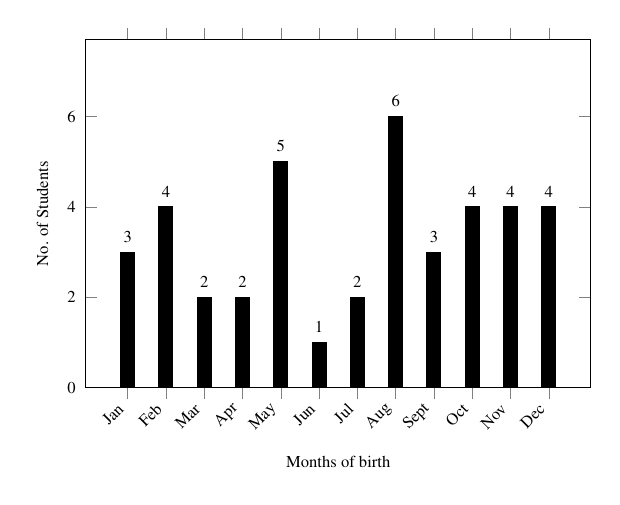
\begin{tikzpicture}


\begin{axis}[
ybar,
ymin=0,
width=8cm,
height=6cm,
ymax=7,
bar width=5pt,
ylabel={No. of Students},
xlabel={Months of birth},
nodes near coords,
symbolic x coords={Jan,Feb,Mar,Apr,May,Jun,Jul,Aug,Sept,Oct,Nov,Dec},
xtick = data,
x tick label style={rotate=45,anchor=east},
enlarge y limits={value=0.1,upper},
legend pos=north east,
]
\addplot[fill=black] coordinates {(Jan,3) (Feb,4)(Mar,2) (Apr,2)(May,5)(Jun,1)(Jul,2)(Aug,6)(Sept,3)(Oct,4)(Nov,4)(Dec,4)};
\end{axis}
\end{tikzpicture}
    
    Find the probability that a student of the class was born in August.\\
\item Three coins are tossed simultaneously 200 times with the following frequencies of different outcomes:\\

\resizebox{\columnwidth}{10pt}{%
\begin{tabular}{ |c|c|c|c|c| } 
 \hline
 \textbf{Outcome} &3 heads &2 heads &1 head &No head\\ 
 \hline
 \textbf{Frequency}  &23 &72 &77 &28\\ 
 \hline
\end{tabular}%\\
}\\

If the three coins are simultaneously tossed again, compute the probability of 2 heads coming up.\\
\item Refer the table given below.\\
\begin{tabular}{ |c|c| } 
 \hline
 \textbf{Marks} &\textbf{Number of students}\\
 \hline
  0-20 &7\\ 
  20-30 &10\\ 
  30-40 &10\\ 
  40-50 &20\\ 
  50-60 &20\\ 
  60-70 &15\\ 
  70-above &8\\ 
  \hline
 \textbf{Total}  &90\\ 
 \hline
\end{tabular}\\

(i) Find the probability that a student obtained less than 20$\%$ in the mathematics test.\\
(ii) Find the probability that a student obtained marks 60 or above.\\




\item To know the opinion of the students about the subject statistics, a survey of 200 students was conducted. The data is recorded in the following table.\\
\begin{tabular}{ |c|c| } 
 \hline
 \textbf{Opinion} &\textbf{Number of students}\\
 \hline
 like  &135\\ 
 dislike  &65\\ 
 \hline
\end{tabular}\\
Find the probability that a student chosen at random\\
(i)likes statistics,\\
(ii) does not like it.\\
\item Refer the table below\\

\begin{tabular}{ cccccccccc} 

 5 &3 &10 &20 &25 &11 &13 &7 &12 &31\\
 19 &10 &12 &17 &18 &11 &32 &17 &16 &2\\
 7 &9 &7 &8 &3 &5 &12 &15 &18 &3 \\
 12 &14 &2 &9 &6 &15 &15 &7 &6 &12\\ 
 \end{tabular}\\

What is the empirical probability that an engineer lives:\\
(i) less than 7 km from her place of work?\\
(ii)more than or equal to 7 km from her place of work?\\
(iii) within $\frac{1}{2}$km from her place of work?\\

\item An organisation selected 2400 families at random and surveyed them to determine a relationship between income level and the number of vehicles in a family. The information gathered is listed in the table:\\
\ref{multicolumn_table}
\begin{table}
\begin{tabular}{|c|c|c|c|c|}
\hline
\textbf{Monthly income} &\multicolumn{4}{c|}{\textbf{vehicles per family }}\\
\cline{2-5}
(in \textbf{\rupee}) &\textbf{0} &\textbf{1} &\textbf{2} &\textbf{Above 2}\\
\hline
Less than 7000 &10 &160 &25 &0\\
\hline
7000-10000 &0 &305 &27 &2\\
\hline
10000-13000 &1 &535 &29 &1\\
\hline
13000-16000 &2 &469 &59 &25\\
\hline
16000 or more  &1 &579 &82 &88 \\
\hline
\end{tabular}
\end{table}\\
Suppose a family is chosen.Find the probability that the family chosen is\\
(i) earning \rupee 10000 – \rupee 13000 per month and owning exactly 2 vehicles.\\
(ii) earning \rupee 16000 or more per month and owning exactly 1 vehicle.\\
(iii) earning less than \rupee 7000 per month and does not own any vehicle.\\
(iv) earning \rupee 13000 – \rupee 16000 per month and owning more than 2 vehicles.\\
(v) owning not more than 1 vehicle.\\

\item Eleven bags of wheat flour, each marked 5 kg, actually contained the following weights of flour (in kg):\\
4.97 5.05 5.08 5.03 5.00 5.06 5.08 4.98 5.04 5.07 5.00\\
Find the probability that any of these bags chosen at random contains more than 5 kg of flour.\\

\item Prepare a frequency distribution table, regarding the concentration of sulphur dioxide in the air in parts per million of a certain city for 30 days.\\

\begin{tabular}{ cccccc} 

  0.03 &0.08 &0.08 &0.09 &0.04 &0.17 \\
 0.16 &0.05 &0.02 &0.06 &0.18 &0.20 \\
 0.11 &0.08 &0.12 &0.13 &0.22 &0.07  \\
 0.08 &0.01 &0.10 &0.06 &0.09 &0.18 \\ 
  0.11 &0.07 &0.05 &0.07 &0.01 &10.04 \\ 
 \end{tabular}\\
  Using this table, find the probability of the concentration of sulphur dioxide in the interval 0.12 - 0.16 on any of these days.\\
\item  
A, B, O, O, AB, O, A, O, B, A, O, B, A, O,\\ O,
A, AB, O, A, A, O, O, AB, B, A, O, B, A, B, O.\\
prepare a frequency distribution table regarding the blood groups of 30 students of a class. Use this table to determine the probability that a student of this class, selected at random, has blood group AB.\\

\end{enumerate}
\end{document}
